% #############################################################################
% This is Chapter 1
% !TEX root = ../main.tex
% #############################################################################
% Change the Name of the Chapter i the following line
\chapter{Introduction}
% The following line allows to ref this chapter
\label{chap:intro}

The continuous growth and expansion of the world population and the correspondent increase of energy needs, is one of the most relevant topics of the century. The issues caused by the increasing usage of fossil fuels and the amount of carbon dioxide produced everyday is affecting our lives and the future of the planet. In 2019, Industry and buildings account for over 90\% of global electricity demand today, while transport makes up less than 2\% \cite{iea}. Recent studies show that the building sector represents 39\% and 40\% of the energy consumption and 38\% and 36\% of the CO2 emissions in the U.S. \cite{CivilUS} and Europe\cite{CivilEU}, respectively. The expansion of office buildings and the multiplication of the amount of energy needed in order to satisfy the demands of a society that is becoming more and more technologically dependent, are two catalysts for the recent increase of energy consumption. 



On the other hand, sustainable alternatives have also emerged to replace some less ecological social habits. Electric cars are the best example of this. The adoption of electric cars is a practice that has been increasing in the last decade and is expected to grow even more in the next two. Currently the major limitation is the autonomy of the cars, since the batteries still do not have, in most cases, enough capacity to equal the autonomy performance of a fuel car. In this sense, a solution that has been adopted is the installation of charging stations in both residential and office buildings. According to \cite{charger}, the infrastructure for electric-vehicle charging is expanding and in 2019, there were about 7.3 million chargers worldwide, of which about 6.5 million were private. The energy spent on charging electric cars in buildings is a new factor to be studied, both in the influence it has on the energy consumption of the building and the reduction of energy waste while using it.


The extent of available data is also multiplying, and the analysis and modeling of this data is becoming essential to minimize energy waste. Modern infrastructures are already equipped with systems able to monitor and control power usage, and there has been an increase in the number of chargers for electric cars installed in garages. The technology also evolved to allow buildings to produce their own energy. The implementation of \ac{PV} panels in buildings is an increasingly common practice. Despite the low efficiencies (from 15\% to 17\% \cite{pv}), \ac{PV} panels are becoming an important energy source for buildings, both  residential and non-residential. 

Modeling energy consumption behaviour and identifying patterns can be crucial to optimize energy usage, and to develop new methodologies to optimize resources. Figure \ref{consumption} illustrates the energy consumption profile of \ac{EDP}'s building in Lisbon, Portugal, between January 25, 2020 and March 13, 2020. In Figure \ref{production}, we may see the production profile for the same building and time-interval as Figure \ref{consumption}. The \ac{PV} behaviour is also cyclical but presents a daily period due to the fact that solar radiation is not influenced by the day of the week.





\begin{figure}[h!]
\captionsetup[subfigure]{position=b}
\centering
\subcaptionbox{\label{consumption}}{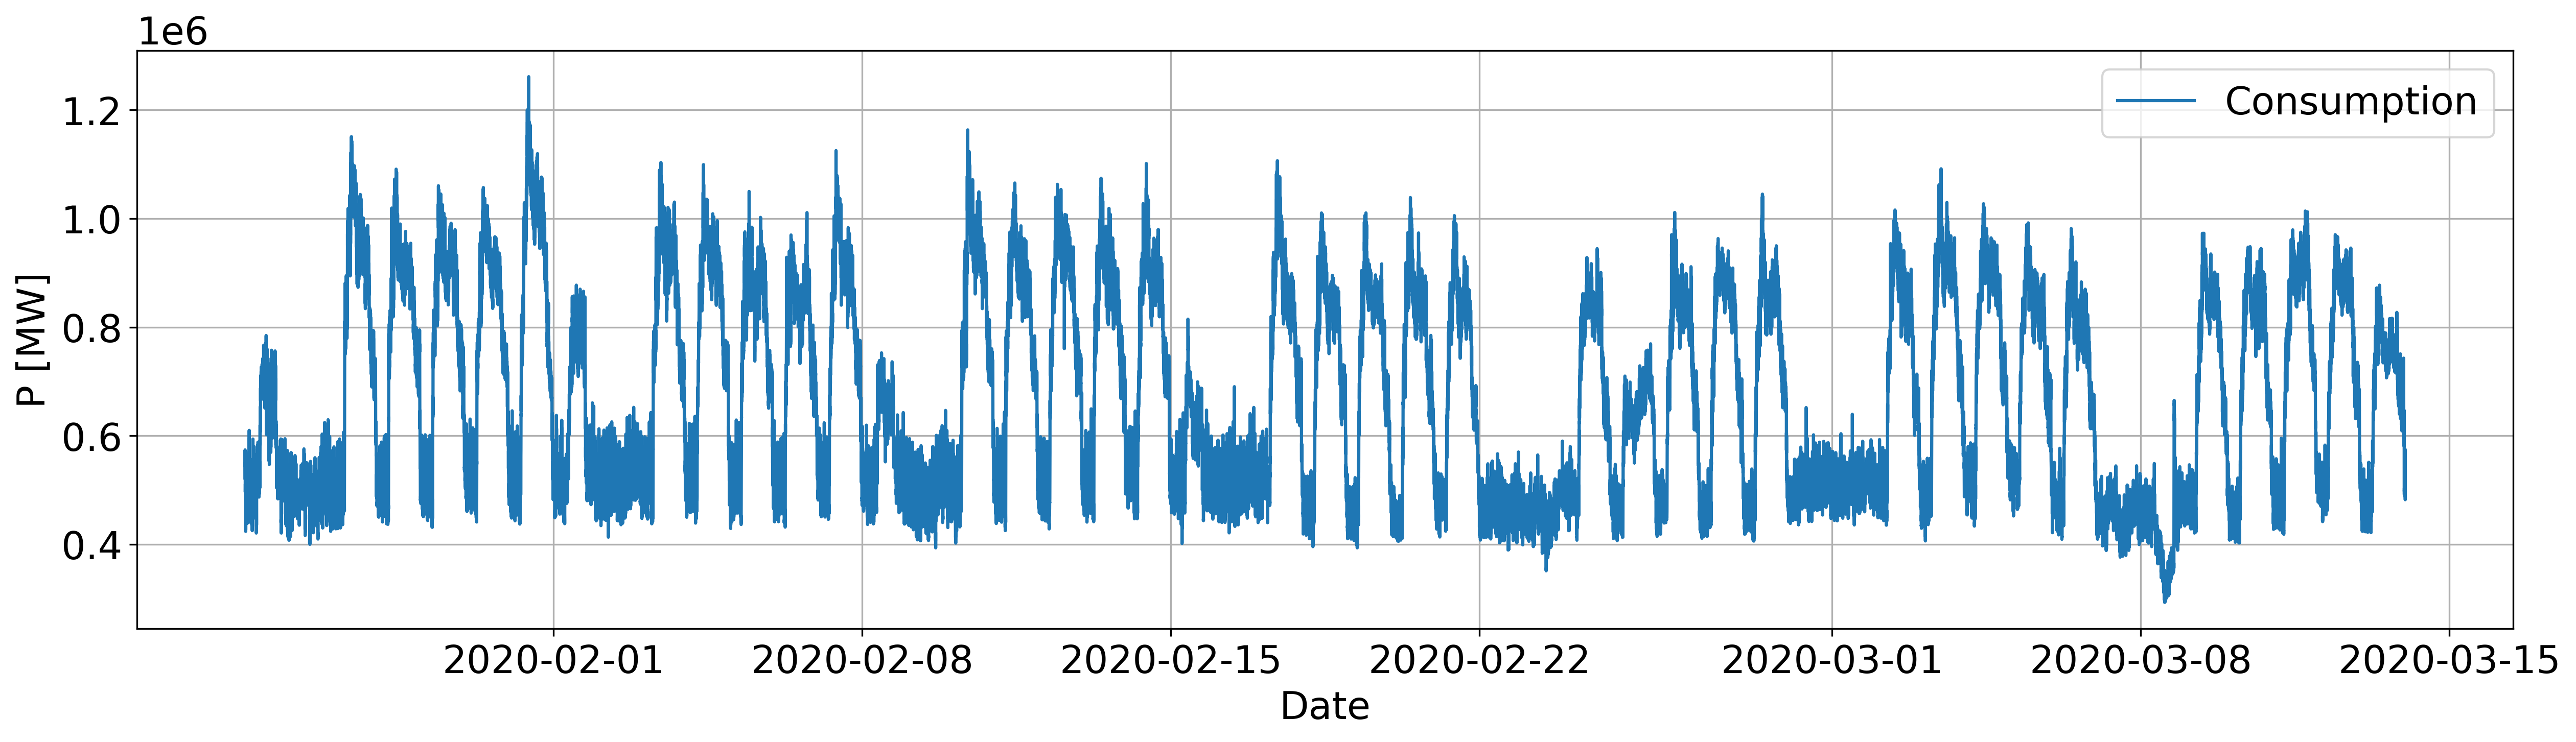
\includegraphics[width=0.9\linewidth]{Images/Consumption_Trend.png}}
\hspace{0.05\textwidth}
\subcaptionbox{ \label{production}}{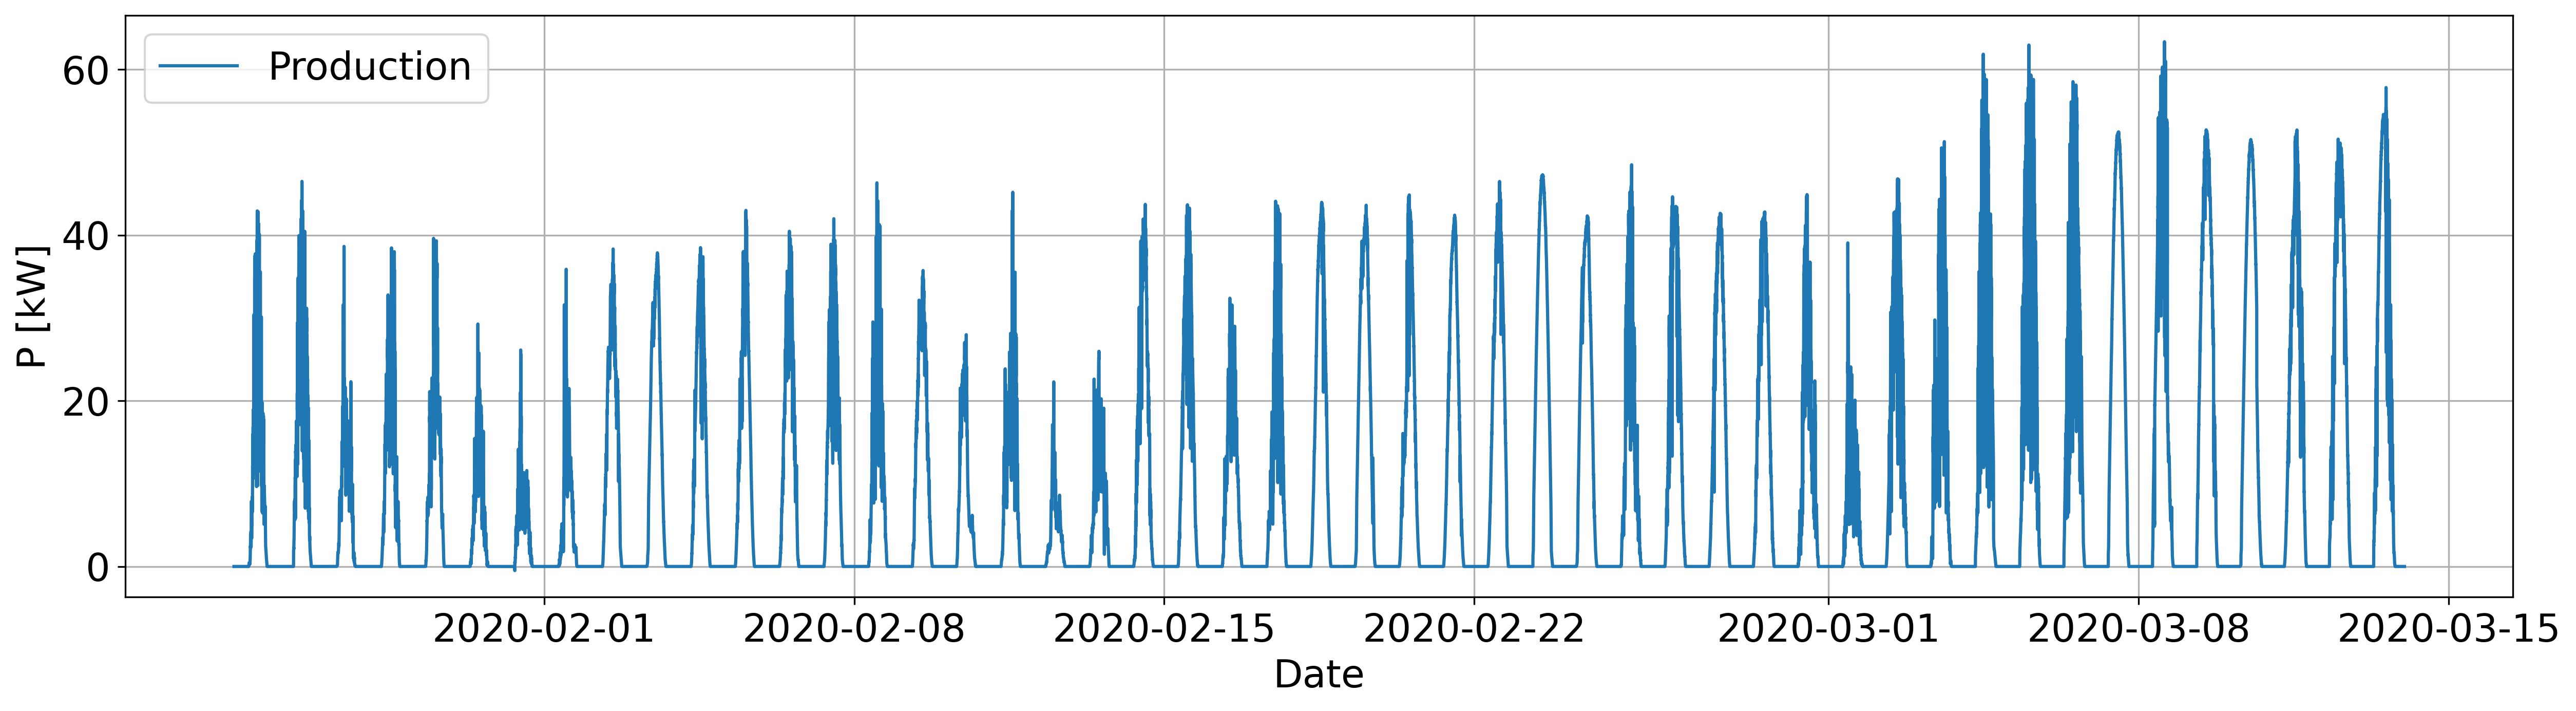
\includegraphics[width=0.9\linewidth]{Images/Production_Trend.png}}
\caption{EDP's building's a) consumption and b) production trends.}
\end{figure}


The profile illustrated in Figure \ref{consumption} shows a movement that one can identify as a trend. The data presented provides power consumption details of 7 weeks and 7 weekends. The behaviour of the profile tends to be cyclical with a 7 day period.

Power consumption forecasting for buildings is a well know area of research. According to \cite{CivilEU}, Energy consumption forecasting plays a significant role in plans to improve energy performance, save energy and reduce the hazardous environmental impact. Moreover, forecasting also plays a vital role in decision-making and future planning which rely on accurate forecasting result. The ability to predict energetic usage of any building has many interesting utilities. Both power consumption and power production are vital information to have in order to predict power available at each time in the building. With this information, there are multiple innovative ideas that can be implemented with the goal of having a more sustainable and power-optimized building, such as electrical vehicle charging.   



\section{Problem statement and objectives}


\ac{EDP} is a vertically integrated energy company with a consolidated position in the Iberian Peninsula, both in terms of electricity generation, distribution and supply, and gas supply. \ac{EDP}'s building in Lisbon, Portugal is equipped with 70 kWp (kilowatt “peak”) of solar generation. Additionally, there are several electric vehicle \ac{EV} charging stations divided in three types:

\begin{enumerate}[noitemsep,topsep=0pt]
  \itemsep0em 
  \item “Dummy” charging stations, which possess no means of intercommunicating with other \ac{IT} devices and have a constant charging rate;
  \item\label{two} “Smart charging” stations, which can vary their power output and suppress the \ac{EV}s’ demands, depending on the global consumption of \ac{EDP}'s building;
  \item “Vehicle2Grid” stations, which charge the vehicle and use the energy stored in the vehicle when the building energy demand spikes..
\end{enumerate} 

This thesis focuses on point \ref{two} - “Smart Charging” stations and aim to enrich \ac{EDP}’s “Smart Charging Hub”. 

The ability to forecast building power consumption's and the respective power available at each time, can be decisive to optimize power usage in a building.  


Regarding energy profile, there are two main types of buildings, residential buildings and non-residential buildings. A building should be regarded as residential building when more than half of the floor area is used for dwelling purposes \cite{OECD}. On the other hand, non-residential buildings consists of buildings other than dwellings, including fixtures, facilities and equipment that are integral parts of the structures and costs of site clearance and preparation \cite{OECD}. The work presented focuses on non-residential buildings, more specifically office buildings.

 




The main task is to answer one simple question: "How can one forecast the amount of energy available in a near future, in order to optimize the energy used in electrical vehicles \ac{EV} smart charging stations?".


The objective is to create a predictive model capable of relating the production and energy consumption of the building, compute and predict the energy available in the future and use that forecast to feed the "Intelligent Central Loading System \ac{EV}" to act accordingly and translate useful data into "\ac{EV} loading orders". 


In other words, the goal is to define a short-term power availability forecast algorithm to help smart-buildings manage power supply for "\ac{EV} Smart Charging Stations".
The expected result of the research should be (but not limited to) a maximum and minimum power output forecast algorithm to boost the capabilities of the “\ac{EV} Smart Charging Central System” by predicting \ac{EDP}'s building power demand worst-case scenario for the next 5, 10 and/or 15 minutes:
\begin{enumerate}[noitemsep,topsep=0pt]
  \itemsep0em 
  \item Make predictions and compare the results for different time-frames (5, 10 and 15 minutes);
  \item Serve the power demand prediction outputs as inputs for a decision-based algorithm to act directly on the “\ac{EV} Smart Charging” Stations.
\end{enumerate}   
  
The challenge of this task lies in finding a system capable of producing a sufficiently precise solution in an acceptable time span, and it was based on these two premises that all the work of this thesis was developed.

\section{Thesis outcome}


There are numerous techniques used in time series forecasting and reach a future consumption value. These techniques are divided into three major groups, the statistical models, the engineering models and the machine learning models. This thesis proposes solutions of the third group, machine learning, that aim to predict the energy available in 5, 10 and 15 minutes in the future

In the process of carrying out this research, meteorological and radiation data provided by the Faculty of Sciences of the University of Lisbon were used, as well as data regarding the energy production and consumption of the building, provided by \ac{EDP}.
Since it is a building with \ac{PV} panels, we can divide the work done in two stages:
\begin{enumerate}[noitemsep,topsep=0pt]
  \itemsep0em 
  \item Data prepossessing;
  \item Treatment and importance of energy production data for the forecasting task;
  \item Creation of a production and consumption forecast model.
\end{enumerate}



In Figure  \ref{scope} it is possible to observe a representation of the objective of this thesis. This figure aims to summarize the whole process of the work developed as well as to clarify what is inside and outside the scope of the proposed challenge.

\begin{figure}[h!]
    \centering
    \begin{center}
    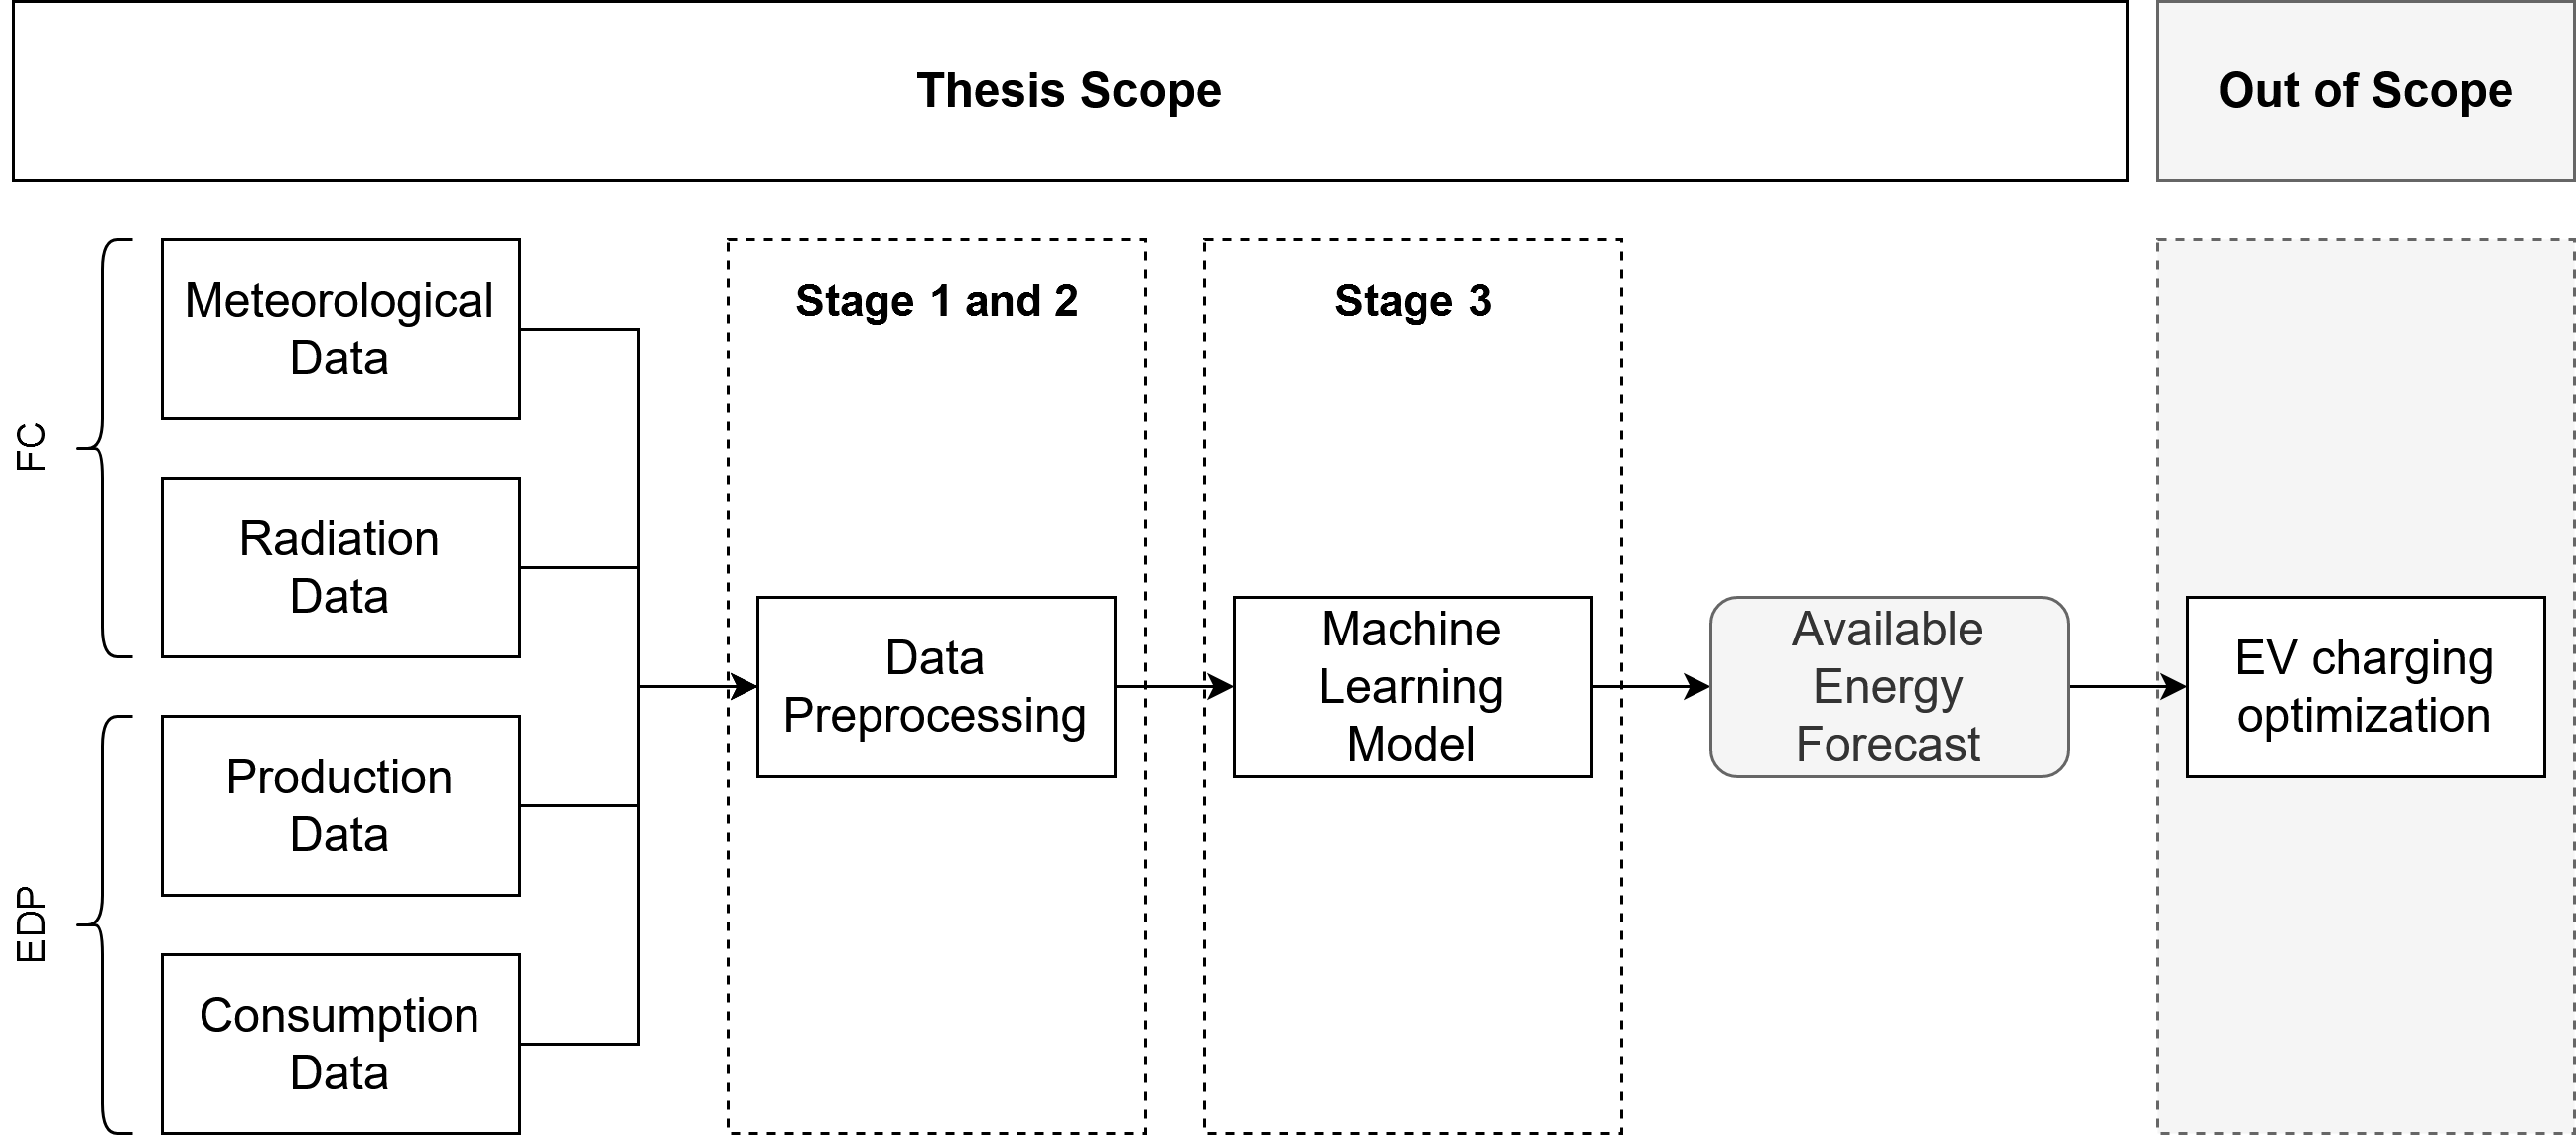
\includegraphics[width=1\textwidth]{Images/Thesis_objective.png}
    \caption{Thesis Scope.}
    \label{scope}
    \end{center}
\end{figure}

As can be seen in Figure \ref{scope}, the purpose of this thesis is to implement a model capable of computing the available energy in the near future. Knowing the maximum energy available for the building, adding the forecast of the energy produced by the \ac{PV} panels and subtracting the forecast of the energy consumed, it is possible to obtain the energy that is ready to be used in the charging of electric vehicles. Outside the context of this work is the use of these forecasts for the construction of optimization models of the charging points. 

It is the combination of all these stages that allows us to perform the proposed task. In total, data ranging from January 2020 to October 2020 was used.





\section{Thesis Outline}